\documentclass[10pt,a4paper,twocolumn]{article}
\newcommand\tab[1][0.5cm]{\hspace*{#1}}
\title{%
	ROS: Robot Localization \\
	\large Course assignment: Intelligent Agents and Robotic Systems \\
	University of Piraeus, Demokritos}
\author{
	Papadopoulos, Vasileios\\
	\texttt{vassilispapadop@gmail.com}
}

\usepackage[utf8]{inputenc}
\usepackage[T1]{fontenc}
\usepackage{amsmath}
\usepackage{amsfonts}
\usepackage{amssymb}
\usepackage{graphicx}
\usepackage{amsmath}
\usepackage{graphicx}
\usepackage{hyperref}
\graphicspath{ {./images/} }


\begin{document}
\maketitle
	
\section{Introduction}
Robot localization is a process to examine the exact position within its environment; Navigation is a crucial activity for a mobile robot for safety, operation and other reasons. A mobile robot needs to know not only its \textit{absolute} position but also its \textit{relative} position in respect, for example to a human who might interact with it. Navigation process requires 4 building blocks; \textit{Perception}, \textit{Localization}, \textit{Congition} and \textit{Motion Control}.


\section{Methods}

The \textit{robot\textunderscore localization\textunderscore demo.launch} file consists of total 6 nodes.

\begin{itemize}
	\item turtlesim node: displays real turtle's measurements and estimated position
	\item turtle1\textunderscore position\textunderscore system\textunderscore node: adds noise to the position of the turtle at a given frequency
	\item turtle1\textunderscore odomentry\textunderscore node: adds noise to the movements of the turtle at a given frequency
	\item robot\textunderscore localization\textunderscore ekf\textunderscore node\textunderscore odom: Extended Kalman Filter to odometry frame
	\item robot\textunderscore localization\textunderscore ekf\textunderscore node\textunderscore map: Extended Kalman Filter to map frame
	\item transformation\textunderscore visualiazation\textunderscore node: Visualization of estimated position in map frame
\end{itemize}

In order to point out the differences between robot\textunderscore localization\textunderscore ekf\textunderscore node\textunderscore odom and robot\textunderscore localization\textunderscore ekf\textunderscore node\textunderscore map we need to briefly describe \textit{Kalman Filter} and \textit{extended Kalman Filter}. Kalman Filter, is an iterative mathematical process that uses set of equations and consecutive data inputs to estimate values such as: position and velocity of an object when the measured values contain unpredicted or random error, uncertainty or variation. The Kalman Filter does not \textit{wait} for a bunch of input data to make an estimate(for example, average) instead, it makes a quick prediction/estimate from few data points by \textit{undestanding} the variation or the uncertainty in them. Generally, the input data are not the true value but something around the true value, Kalman Filter is a process of estimating the true value \textit{real time}. The extended version of the process, models the added noise as a non-linear function.

Both EKF nodes are operating at the same frequency 10Hz which is the rate of producing a state estimate. Also, they have the same sensor\textunderscore timeout. The differences lie onto where the filter is making an estimate. In the first case, it estimates the odom frame while in second the map frame.

To perform our experiments we made some preliminary changes to the original demo. At first step, we launched the robot\textunderscore localization \textunderscore robot package and recorded a \textit{rosbag} of approximately for 35 seconds passing the parameter \textit{-a} to capture all available topics. This recording is used for the carried experiements, which will be present in later sections. Then, we cloned the robot\textunderscore localization \textunderscore demo.launch file into {mylaunch.launch} and removed the node with name \textit{teleop}, type \textit{turtle\textunderscore teleop\textunderscore key} from package \textit{turtlesim} to prevent keyboard teleoperation. Within the newly created launch file, we added a new node from the package \textit{rosbag}, type \textit{play} and passed the path of the previous rosbag. Now, everytime we launch the \textit{mylaunch.launch} file the simulation immediatelly starts playing the rosbag file. We ran 6 different cases. This step is referred as \textit{baseline} in which we simply replay the rosbag mentioned above. The other five cases are presented in the Table 1 below.

\begin{table*}[ht]
	\centering
	\begin{tabular}{|c c c|} 
		\hline
		& Parameters & Node  \\ [0.1ex] 
		\hline\hline
		1) Baseline & default parameters  & -  \\
		2) Position Sensor Noise & -f 1. -x 0.5 -y 0.5 -t 0.2 -v  & turtle1\textunderscore positioning\textunderscore system\textunderscore node  \\
		3) Velocity Sensor Noise & -f 20. -x 0.1 -X 0. -t 0. -T 0.02 -v  & turtle1\textunderscore odometry\textunderscore node  \\
		4) Sensors Sampling Rate & -f 1.8 -x 0.2 -y 0.2 -t 0.2 -v  & turtle1\textunderscore positioning\textunderscore system\textunderscore node  \\
		4) Sensors Sampling Rate & -f 10. -x 0.05 -X 0. -t 0. -T 0.02 -v  & turtle1\textunderscore odometry\textunderscore node   \\
		5) EKF Frequency & 20Hz  & robot\textunderscore localization\textunderscore ekf\textunderscore node\textunderscore odom \\
		5) EKF Frequency & 5Hz & robot\textunderscore localization\textunderscore ekf\textunderscore node\textunderscore map  \\ [1ex] 
		\hline
	\end{tabular}
	\caption{Test cases \label{overflow}}
\end{table*}
	
	
\begin{figure}[ht!]
	\centering
	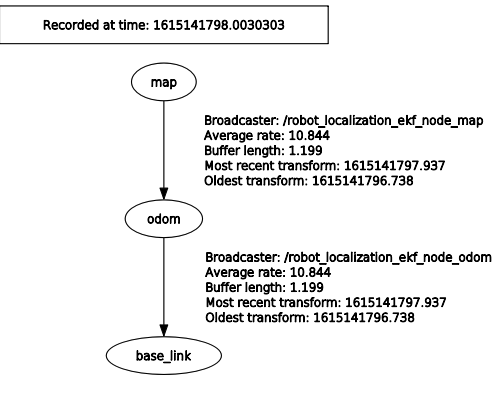
\includegraphics[width=70mm]{rqt_tf_tree}
	\caption{rqt tf tree \label{overflow}}
\end{figure}	
	
\section{Results}

In this section we present the results of previous test cases. The simulation consists of 4 turtles. The turtle with \textit{gray} line is the real turtelsim robot. The position sensor which measures the absolute position and orientation is drawn with \textit{blue} line while the turtle which measures the linear and angular velocity is shown in \textit{red} line. Finally, the \textit{green} line represents the estimate of the pose in map frame.

\begin{figure}[ht!]
	\centering
	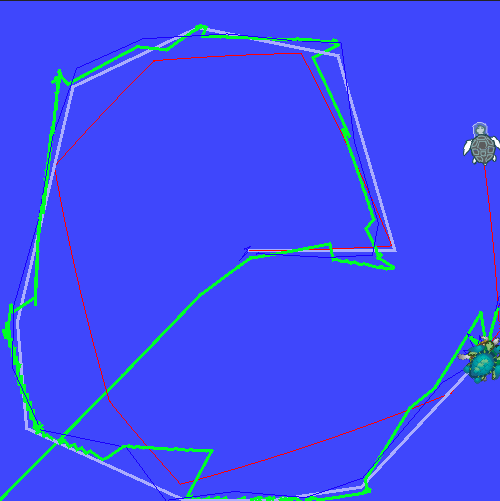
\includegraphics[width=70mm]{baseline}
	\caption{Baseline path \label{overflow}}
\end{figure}

In Figure 2, the baseline case we could track the \textit{red} line and how it starts to drift apart. Red line estimates pose in the map frame by odom frame. The accumulated error becomes clearly visible.

\begin{figure}[ht!]
	\centering
	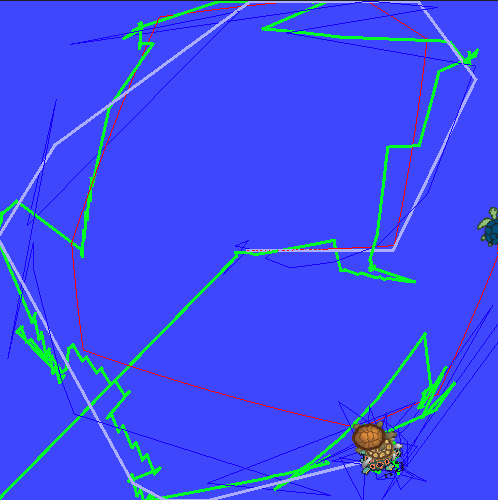
\includegraphics[width=70mm]{position_sensor_noise}
	\caption{Path after position sensor noise \label{overflow}}
\end{figure}

In Figure 3, in contrast to baseline case we have increased the noise in position sensor. Particularly, the standard deviation in X and Y have increased from 0.2 units to 0.5 units per measurement. We observe a pattern seems to follow, loosely speeking the actual position of the turtle though, it jumps randomly quite a bit.

\begin{figure}[ht!]
	\centering
	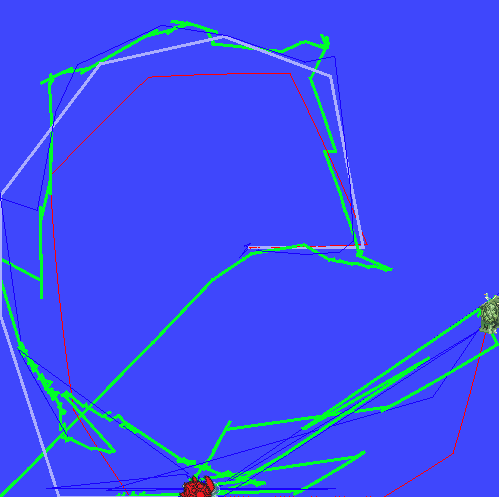
\includegraphics[width=70mm]{velocity_sensor_noise}
	\caption{Path after velocity sensor noise \label{overflow}}
\end{figure}

In Figure 4, we doubled the linear velocity error from 0.05 to 0.1.

\begin{figure}[ht!]
	\centering
	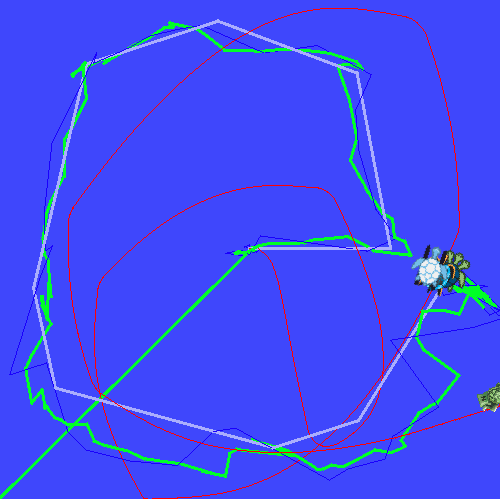
\includegraphics[width=70mm]{sampling_rate}
	\caption{Path after sampling rate change \label{overflow}}
\end{figure}

\begin{figure}[ht!]
	\centering
	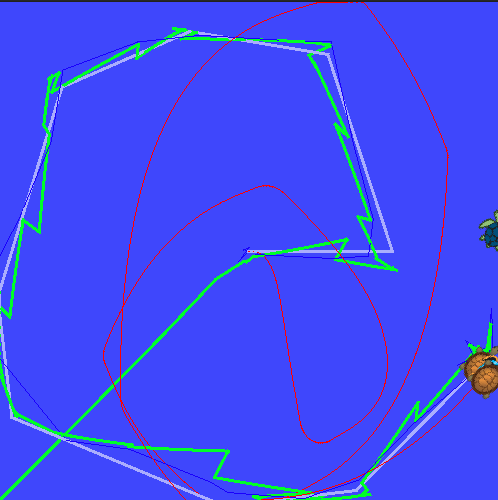
\includegraphics[width=70mm]{ekf_frequency}
	\caption{Path after EFK frequency change \label{overflow}}
\end{figure}

In Figures 5 and 6 we tested the behaviour of the system when changing sensors sampling rate and the frequency the 2 EKF nodes make an estimate. In Figure 5 the red line shows much greater drift from the odometry sensor with half the sampling rate 10Hz.


\section{5.a}
map-frame$\leftarrow$odom-frame$\leftarrow$base-link. Both \textit{map-frame} and \textit{odom-frame} are world fixed frames. Though, odometer will drift and accumulate error. To fix this we need to publish a map to odom transformation which will essentially fix the pose of the robot in the map frame.

\section{5.b}

\begin{thebibliography}{9}
	\bibitem{moore} 
	Thomas Moore and Daniel Stouch. 
	\textit{A Generalized Extended Kalman Filter Implementation for the Robot Operating System}. 
	Sensor Processing and Networking Division Charles River Analytics, Inc. Cambridge, Massachusetts, USA.	
	
\end{thebibliography}


	
\end{document}